\documentclass[border=2pt]{standalone}
\usepackage{tikz}
\usetikzlibrary{matrix,positioning,arrows.meta,arrows,calc}

\tikzset{
mymat/.style={
  matrix of math nodes,
  text height=2.5ex,
  text depth=0.75ex,
  text width=5.25ex,
  align=center,
  column sep=-\pgflinewidth
  },
mymats/.style={
  mymat,
  text width=8ex,
  nodes={draw}
  }  
}
\begin{document}

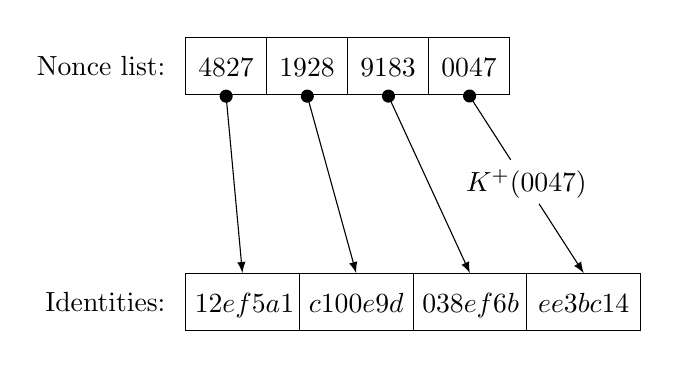
\begin{tikzpicture}[>=latex]
\matrix[mymat,anchor=west,row 1/.style={nodes=draw}]
at (0,0) 
(mat1)
{
4827 & 1928 & 9183 & 0047\\
};
\matrix[mymats=white,anchor=west]
at (0,-3) 
(mat3)
{
12ef5a1 & c100e9d & 038ef6b & ee3bc14 \\
};

\node[left=0pt of mat1]
  (cella) {Nonce list:};
  
\node[left=0pt of mat3]
  (cella) {Identities:};
  
  
\node (key) at ($(mat1-1-4.south)!0.5!(mat3-1-4.north)$) {$K^+(0047)$};

\begin{scope}[shorten <= -2pt]
\draw[*->]
  (mat1-1-1.south) -- (mat3-1-1.north);
\draw[*->]
  (mat1-1-2.south) -- (mat3-1-2.north);
\draw[*->]
  (mat1-1-3.south) -- (mat3-1-3.north);
\draw[*-]
  (mat1-1-4.south) -- (key);
\draw[->]
  (key) -- (mat3-1-4.north);
\end{scope}
\end{tikzpicture}

\end{document}